\setAuthor{Kaur Aare Saar}
\setRound{lõppvoor}
\setYear{2023}
\setNumber{G 5}
\setDifficulty{5}
\setTopic{TODO}

\prob{Sundventilatsioon}
Maril on kodus sundventilatsioon. Ta avastas, et ta peab õhuniisutit, mille paaki mahub $m=\SI{1}{\kg}$ vett, täitma iga kümne tunni tagant selleks, et hoida toas suhtelist õhuniiskust $r_1= 50 \%$. Väljas on temperatuur $T_2 = \SI{-5}{\celsius}$ ja suhteline õhuniiskus $r_2 = 80 \%$ ning toas on temperatuur $T_1= \SI{20}{\celsius}$. Kasutades juuresolevat küllastunud aururõhu graafikut, leidke mis kiirusega vahetab sundventilatsioon toas olevat õhku. Vee molaarmass on $M=\SI{18}{\gram\per\mole}$, gaasi universaalkonstant $R=\SI{8.31}{\joule\per\mole\per\kelvin}$ ja õhurõhk on $p=\SI{100}{\kilo\pascal}$.
\begin{center}
  \vspace{-2em}
  \pgfkeys{/pgf/number format/.cd,1000 sep={}}% Suurtes arvudes komasid pole selguse huvides
  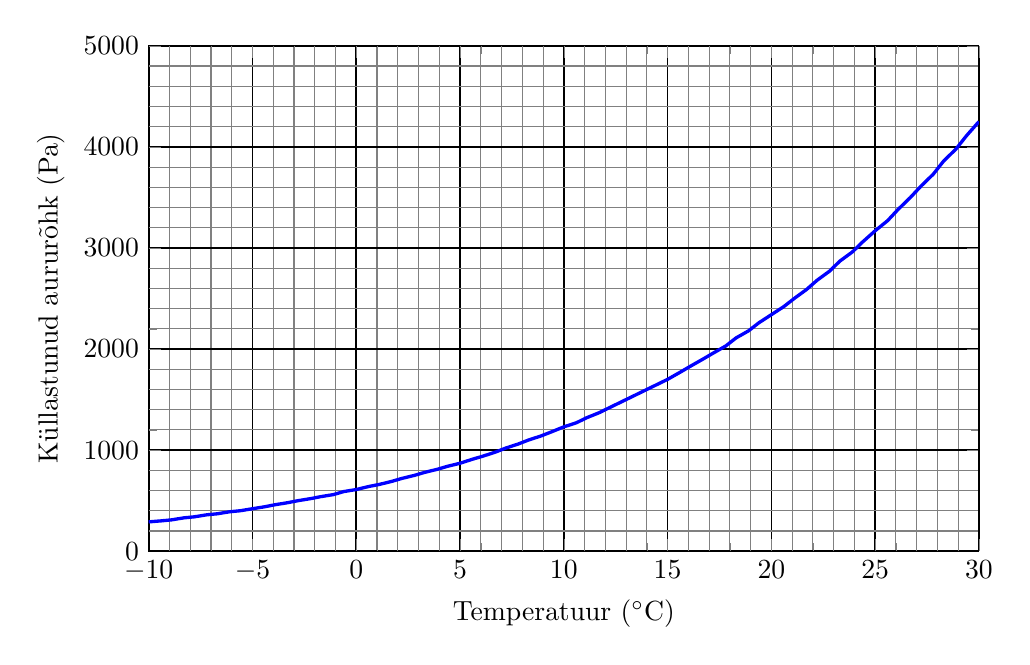
\begin{tikzpicture}
    \begin{axis}[
      xlabel={Temperatuur ($^\circ$C)},
      ylabel={Küllastunud aururõhk (Pa)},
      xmin=-10, xmax=30,
      ymin=0, ymax=5000,
      xtick={-10,-5,0,5,10,15,20,25,30},
      ytick={0,1000,2000,3000,4000,5000},
      minor tick num=4,
      grid=both,
      minor grid style={thin,gray},
      major grid style={semithick,black},
      width=\textwidth,
      height=8cm,
      ]

      \addplot[color=blue,very thick]
      coordinates {
        (-10.00,290.0)
        (-9.40,300.0)
        (-8.90,310.0)
        (-8.30,330.0)
        (-7.80,340.0)
        (-7.20,360.0)
        (-6.70,370.0)
        (-6.10,390.0)
        (-5.60,400.0)
        (-5.00,420.0)
        (-4.40,440.0)
        (-3.90,460.0)
        (-3.30,480.0)
        (-2.80,500.0)
        (-2.20,520.0)
        (-1.70,540.0)
        (-1.10,560.0)
        (-0.60,590.0)
        (0.00,610.0)
        (0.60,640.0)
        (1.10,660.0)
        (1.70,690.0)
        (2.20,720.0)
        (2.80,750.0)
        (3.30,780.0)
        (3.90,810.0)
        (4.40,840.0)
        (4.40,840.0)
        (5.00,870.0)
        (5.60,910.0)
        (6.10,940.0)
        (6.70,980.0)
        (7.20,1020.0)
        (7.80,1060.0)
        (8.30,1100.0)
        (8.90,1140.0)
        (9.40,1180.0)
        (10.00,1230.0)
        (10.60,1270.0)
        (11.10,1320.0)
        (11.70,1370.0)
        (12.20,1420.0)
        (12.80,1480.0)
        (13.30,1530.0)
        (13.90,1590.0)
        (14.40,1640.0)
        (15.00,1700.0)
        (15.60,1770.0)
        (16.10,1830.0)
        (16.70,1900.0)
        (17.20,1960.0)
        (17.80,2030.0)
        (18.30,2110.0)
        (18.90,2180.0)
        (19.40,2260.0)
        (20.00,2340.0)
        (20.60,2420.0)
        (21.10,2500.0)
        (21.70,2590.0)
        (22.20,2680.0)
        (22.80,2770.0)
        (23.30,2870.0)
        (23.90,2960.0)
        (24.40,3060.0)
        (25.00,3170.0)
        (25.60,3270.0)
        (26.10,3380.0)
        (26.70,3500.0)
        (27.20,3610.0)
        (27.80,3730.0)
        (28.30,3860.0)
        (28.90,3980.0)
        (29.40,4110.0)
        (30.00,4250.0)
      };
    \end{axis}
  \end{tikzpicture}
  \vspace{-3em}
\end{center}


\hint

\solu
\par
Loeme juuresolevalt graafikult, et temperatuuril $T_1 = \SI{20}{\celsius}$ on küllastunud aururõhk $p_{k1} = \SI{2340}{\pascal}$ ja temperatuuril $T_2 = \SI{-5}{\celsius}$ on küllastunud aururõhk $p_{k2} = \SI{420}{\pascal}$. Järelikult on toas veeauru osarõhk $p_1 = p_{k1} r_1 = \SI{1170}{\pascal}$ ja õues on veeauru osarõhk $p_2 = p_{k2} r_2 = \SI{336}{\pascal}$.

Olgu õhu ruumala, mis toast kümne tunni jooksul väljub $V$. Sama palju peab tulema ka sisse.
Toast väljuvas õhus oleva veeauru massi $m_1$ saame arvutada ideaalse gaasi valemist:
$$p_1V = \tfrac {m_1}M RT_1.$$
Ja tuppa sisenevas õhus oleva veeauru koguse $m_2$ saame arvutada valemist:
$$p_2V = \tfrac {m_2}M RT_1.$$
Kuna toas on veeauru hulk konstantne, siis järelikult peab õhuniisutis aurustuma sama palju vett kui palju läheb toast välja. Seega saame seose $m = m_1 - m_2$. Järelikult saame avaldada kümne tunniga toast väljuva õhu ruumala:
$$V = \frac{mRT_1}{M(p_1-p_2)} = \SI{160}{\meter\cubed}.$$
Õhu vahetumise kiiruseks seega saame $\SI{16}{\meter\cubed\per\hour}$.
\probend